\documentclass[12pt, notitlepage]{article}
\usepackage{amsmath}
\usepackage{amssymb}
\usepackage{graphicx}
\usepackage{amsthm}
\usepackage{listings}
\usepackage{color}
\usepackage{float}

\definecolor{dkgreen}{rgb}{0,0.6,0}
\definecolor{gray}{rgb}{0.5,0.5,0.5}
\definecolor{mauve}{rgb}{0.58,0,0.82}

\lstset{
	frame=single,
	language=Java,
	belowskip=3mm,
	showstringspaces=false,
	columns=flexible,
	captionpos=b,
	basicstyle={\small\ttfamily},
	numbers=left,
	numbersep=5pt,
	%numbers=none,
	numberstyle=\tiny\color{gray},
	keywordstyle=\color{blue},
	commentstyle=\color{dkgreen},
	stringstyle=\color{mauve},
	breaklines=true,
	breakatwhitespace=true,
	tabsize=3
}


\providecommand{\abs}[1]{\lvert#1\rvert}
\providecommand{\norm}[1]{\lVert#1\rVert}

\newtheorem{thm}{Theorem}
\newtheorem{lemma}[thm]{Lemma}
\newtheorem{fact}[thm]{Fact}
\newtheorem{cor}[thm]{Corollary}
\newtheorem{eg}{Example}
\newtheorem{ex}{Exercise}
\newtheorem{defi}{Definition}
\newtheorem{hw}{Homework}
\newenvironment{sol}
  {\par\vspace{3mm}\noindent{\it Solution}.}{\qed}

\newcommand{\fib}{\mbox{fib}}
\newcommand{\ov}{\overline}
\newcommand{\cb}{{\cal B}}
\newcommand{\cc}{{\cal C}}
\newcommand{\cd}{{\cal D}}
\newcommand{\ce}{{\cal E}}
\newcommand{\cf}{{\cal F}}
\newcommand{\ch}{{\cal H}}
\newcommand{\cl}{{\cal L}}
\newcommand{\cm}{{\cal M}}
\newcommand{\cp}{{\cal P}}
\newcommand{\cz}{{\cal Z}}
\newcommand{\eps}{\varepsilon}
\newcommand{\ra}{\rightarrow}
\newcommand{\la}{\leftarrow}
\newcommand{\Ra}{\Rightarrow}
\newcommand{\dist}{\mbox{\rm dist}}
\newcommand{\bn}{{\mathbf N}}
\newcommand{\bz}{{\mathbf Z}}

\setlength{\parindent}{0pt}
%\setlength{\parskip}{2ex}
\newenvironment{proofof}[1]{\bigskip\noindent{\itshape #1. }}{\hfill$\Box$\medskip}

\usepackage{enumerate,fullpage, proof}
\newcommand{\Infer}[2]{\infer{#2}{#1}}

\title{Homework 2}
\author{Team: nogg\footnote{E-mail: \texttt{kimi.ysma@gmail.com}}\footnote{Team member: Ma Yesheng, Zhao Ming, Hu Hu, Zou Yikai, Fan Minghua}}

\begin{document}

{\bf\small CS214: Algorithms and Complexity}\hfill{\bf\small 2016 Fall}
{\let\newpage\relax\maketitle}


\begin{ex}\end{ex}
\begin{sol}\\
\textbf{Observation.1} ~We can find that the array A's size is n and n is even, so  we can divide the array into $\frac{n}{2}$ pairs.\\
\textbf{Observation.2} ~If we have two arrays, the biggest number among these arrays must be either the first array's biggest number or the second array's biggest number.\\\\
\emph{step1.} Divide the array into $\frac{n}{2}$ pairs which counts from 1 to $\frac{n}{2}$. \\
\emph{step2.} Inside each pairs we do one comparison to determine which one is bigger and which one is smaller.\\
\emph{step3.} Now we get two arrays, one is composed of the bigger one of each pair, another is composed of the smaller one of each pair.\\
\emph{step4.} Find the biggest number $N_b$ in the first array and the smallest number $N_s$ in the second array.\\
\emph{step5.} Now the biggest number of A is $N_b$ and smallest number of A is $N_s$. \\\\
\textbf{Analysis:}In step2 we do $\frac{n}{2}$ comparisons, and in step4 we do ($\frac{n}{2}$-1)+($\frac{n}{2}$-1).Totally, we do $\frac{n}{2}$ + ($\frac{n}{2}$-1) + ($\frac{n}{2}$-1) = $\frac{3n}{2}$-2 comparisons.
\end{sol}


\begin{ex}\end{ex}
\begin{sol}
\textbf{Observation.}~We have known that we need at least (n-1) times comparisons to find the biggest numbers.\\

\emph{step1.} We find the biggest number in the array through Dividing and Comparing. That is to say, assuming we have a full binary tree which has $2^k$ leaf nodes, and every leaf store a number of the array, and the inside node stores a value which is the bigger one of his sons.\\
So we have to do $(2^{k-1}+2^{k-2}+...+1)$ = $(2^k-1)$ comparisons to find the biggest one. i.e (n-1) comparisons.\\

\textbf{Observation.} The second-biggest number in the array must have done comparison with the biggest one during the construction of the full binary tree.\\
\textbf{Proving.} Assuming the biggest number is $N_1$, and the second-biggest number is $N_2$. If $N_2$ hasn't compared with $N_1$, it must be smaller that a number, and that number is not $N_1$, so $N_2$ is at least third-biggest number, which is not same with the assumption.\\

\emph{step2.} Get the numbers which have compare with $N_1$, there will be $log_2(n)$, which is the height of the full binary tree. Find the biggest number of these $log_2(n)$ numbers.\\

\textbf{Analysis:}~In step1. we do (n-1) comparisons, and in step2. we do ($log_2(n)$-1) comparisons. Totally, we do (n + $log_2(n)$ - 2) comparisons.
\end{sol}


\begin{ex}\end{ex}
\begin{sol}
\textbf{Analysis:}~Given an array A which contains 3 elements $a_1,a_2,a_3$, and these 3 elements is different from each other. According to the given algorithm, we only need one comparison to find the largest number. However, we can compare two elements one time. And no matter how we choose the elements, there is still one element will not be compared and we cannot know whether it is bigger or smaller. So the algorithm is absolutely wrong.
\end{sol}


\begin{ex}\end{ex}
\begin{sol}\\
\textbf{Analysis:} Since we want to get the worst case, which means at every merge level, when one list runs out for adding, the other must have only one element left. Then we can construct the list in this way, which I prefer to call it \textbf{Interpolation}. Now consider the last merge step's reversion: dividing one list(lenth is n) into two lists(lenth is n/2). The interpolation method is to divide it crossways. Assuming the origin list is range(n), then the two new lists are like: [0, 2, 4, ..., n-2] and [1, 3, 5, ...,n-1].Then let's move on, dividing these two lists into four using the same method.Now we can get[0, 4, ..., n-4], [2, 6, ..., n-2], [1, 5, ...,n-3] and [3, 7, ..., n-1].And so on until each list contains only one element, and now explain why it is actually the worst case. If we combine two lists with lenth(n) into one, the elements in previous lists are cross-growing, like a[0]$<$b[0]$<$a[1]$<$b[1]$<$....Then we need $2n-1$ times of addtion to join them. Then we add all the comparion time up, we get $nlogn-n+1$.\\
\textbf{Observation:} Let's denote that the origin list is at level 0, and the two lists are at level 1 and so on. Then we can get that: at level i, the span in each list is $2^i$. And the leaves of this tree is at level log(n), which are lists with only one element.\\
Ok,I think what I explain above is quite enough but not explicit. Let's forget it, I just came up a beautiful and tricky way to construct.\\
\textbf{Process:} If we regard every list(no matter how many elements in it) as a node, then the whole merge process is a \textbf{Full Binary Tree} ,whose leaves are one number and height is log(n)+1. Each node has a unique route from root to it. If at each inner node, the route is gonna choose the left way, then we denote it as 0, right as 1. Then each route has a unique \textbf{binary code}, which is obviously the index of the leaf node in binary. For example, in range(8), leaf no.0's route code is 000 which means left left left, and leaf no.5's route code is 101 which means right left right.In interpolation method, the list's min element will definitely appear in its left child, and max element in its right child. Then we can use this route code plus elements's span in each level to calculate the exact number of each leaf node.\\
\begin{enumerate}[(1)]
\item max=n-1, min=0, span=1, lenth=n, route code=(from $0...0^{logn's}$ to $1...1^{logn's}$), i=logn
\item check if i is now 0, if it is, goto (4),else goto (3)
\item if route code[i]=0, then min remains still, span = span*2, lenth = lenth/2, calculate max by $(max-min)/span + 1 = lenth$, i=i-1, else max remains still, span = span*2, lenth=lenth/2, calculate min by $(max-min)/span + 1 = lenth$, i=i-1. Goto (2)
\item leaf[route code] = min( or max)
\end{enumerate}
\end{sol}


\begin{ex}\end{ex}
\begin{sol}
Let me introduce two methods to solve this problem:\\
\textbf{Method 1:}\\
Let us follow the step we use in class but do more precise work.(Denote that Aii=0 not 1)
\begin{align*}
\sum_{i\neq j}^{}\mathbb{E}[A_{ij}]&=\sum_{i\neq j}^{}\frac{1}{|i-j|+1}\\
&=2\sum_{i=1}^{n}\sum_{l=1}^{n-i+1}\frac{1}{l}-n\\
&=2*(n*1+(n-1)*\frac{1}{2}+...+2*\frac{1}{n-1}+1*\frac{1}{n})-n\\
&=2*((n+1)H_n-n))-2n\\
&=2(n+1)H_n-4n
\end{align*}
\textbf{Method 2:}\\
Let's define that $E_n$ means expected comparisons needed when sorting list with length(n). And since we use kind of shuffle things to choose the pivot, then after  first round comparison, the possibility that the pivot in each position is equal, in other words, $\frac{1}{n}$. And when it's at pos i, then it divides the list into to parts with length{i-1} and {n-i}. Then the total comparison can be represented like this $E_n = E_{i-1}+E_{n-i}+n-1$. In consequence, the expected comparisons is actually $E_n=\frac{1}{n}\sum_{i=1}^{n}(E_{i-1}+E_{n-i}+n-1)$. Now let's do some mathematic things.
\begin{align*}
n*E_n&=2(E_1+E_2+...+E_{n-1})+n(n-1) \tag{1}\\
(n-1)*E_{n-1}&=2(E_1+E_2+...+E_{n-2})+(n-1)(n-2) \tag{2}\\
nE_n&=(n+1)E_{n-1}+2n-2 \tag{(1)-(2)}\\
\end{align*}
Now we can get a series of equations. And then by replacing $E_i$ with $\frac{i+1}{i}E_{i-1}+2-\frac{2}{i}$ until we get:
\begin{align*}
E_n&=\frac{n+1}{2}E_{1}+2(1+\frac{n+1}{n}+...+\frac{n+1}{3})-2(\frac{n+1}{n(n+1)}+\frac{n+1}{n(n-1)}+...+\frac{1}{3*2})\\
&=\frac{n+1}{2}*0+2(n+1)(\frac{1}{3}+\frac{1}{4}+...+\frac{1}{n}+\frac{1}{n+1}-\frac{1}{2}+\frac{1}{n+1})\\
&=2(n+1)(H_n-2+\frac{2}{n+1})\\
&=2(n+1)H_n-4n
\end{align*}
\end{sol}


\begin{ex}\end{ex}
\begin{sol}
In quicksort, we use a pivot number randomly chosen to divide the number sequence ito two part. Then we need to do the same quicksort operation on each part and repeat it. But in quickselect, similarly, in each recursion step, we need to divide the sequence into two part, but we only need to do the same quickselect operation on one of them. Which means that, in quickselect, we only need to do "partial execution" in each step of quicksort. Therefore, quickselectcan be viewed as a "partial execution" of quicksort. \\ \\
We use the sequence \{4, 7, 9, 3, 1, 2, 6, 5, 8\} as an example. The quicksort tree is drawn above.\\
In order to select the $5th$ number in this sequence, the part in red circle is visited by quickselect.
\begin{figure}[H]
	\center
	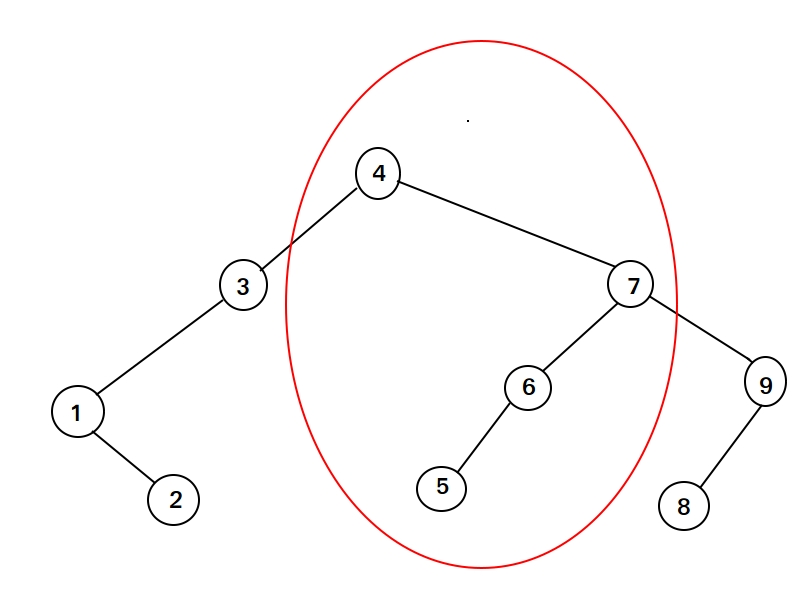
\includegraphics[width=0.8\linewidth]{p1.jpg}\vspace{-10pt}
	\caption{quicksort tree of [4, 7, 9, 3, 1, 2, 6, 5, 8]} \nonumber\label{fig:quicksort tree}\vspace{-10pt}
\end{figure}
\end{sol}


\begin{ex}\end{ex}

\begin{sol}\\

\qquad We want $i$ to be the common ancestor of $j$ and $k$. Consider a sequence which include i, j, k. If we want i be the ancestor of j and k, and assumed i $<$ j $<$ k, we must make sure that the pivot number we choose is j. It means that the pivot we choose must be the second big number in i, j, k.
\[
\mathbb{E}[B_{i, j, k}] = \frac{1}{max\{i,j,k\}-min\{i,j,k\}+1}
\]
\end{sol}


\begin{ex}\end{ex}
\begin{sol}
From analysis of the search route of SelectSort, we can find that the number of comparisons need to do in SelectSort can be counted by all the $i, j, k$ where k is the argument of SelectSort, s.t. $B_{i, j, k} = 1$. Hence, we can define $C(\pi)$ to be:

\[
C(\pi) = \sum_{\substack{i, j\\i\neq j}} B_{i, j, k}
\]

\end{sol}


\begin{ex}\end{ex}
\begin{sol}
With the equation of $C(\pi)$, we can go to compute the expectation of comparisons:
\begin{align*}
\mathbb{E}[C(\pi)] &= \mathbb{E}\left[\sum_{i\neq j} B_{i, j, k}\right] = \sum_{i\neq j}\mathbb{E}[B_{i, j, k}]\\
&= 2 \sum_{i > j}  \mathbb{E}[B_{i, j, k}] = 2(\sum_{\substack{i>j\\1\leq k\leq j}}\mathbb{E}[B_{i, j, k}] + \sum_{\substack{i>j\\j\leq k\leq i}}\mathbb{E}[B_{i, j, k}] + \sum_{\substack{i>j\\i\leq k\leq n}}\mathbb{E}[B_{i, j, k}])  \\
&= 2(\sum_{\substack{i>j\\1\leq k\leq j}}\frac{1}{i-k+1} + \sum_{\substack{i>j\\j\leq k\leq i}}\frac{1}{i - j + 1} + \sum_{\substack{i>j\\i\leq k\leq n}} \frac{1}{k - j + 1}) \\
&=2(\sum_{i = k+1}^{n}\sum_{j=k}^{i-1}\frac{1}{i-k+1}  +  \sum_{i = k+1}^{n}\sum_{j=1}^{k}\frac{1}{i-j+1}       +
\sum_{i=2}^{k}\sum_{j=1}^{i-1}\frac{1}{k-j+1}) \\
&=2\left[ (\sum_{i = 2}^{n-k+1}\frac{i-1}{i}) +
		   (\frac{(n H_n - H_n) - (k H_k - H_k)}{2} + H_n - H_k) + (\sum_{i = 2}^{i = k}\frac{i-1}{i})\right]\\
&\text{(The second term of the above derivation is a little tricky, but if you consider a }\\
&\text{$n\times n$ matrix with each row a harmonic series, it is quite obvious)}\\
& = 2\left[(n-k+1-H_{n-k+1}) + (\frac{(n+1)H_n - (k+1)H_k}{2} + (k-H_k)\right] \\
&= 2(n+1) - 2H_{n-k+1} +(n+1)H_n - (k+3)H_k
\end{align*}
Thus the expectation of comparison number is calculated as above.
\end{sol}

\end{document}
